\chapter{Introduction}\label{Chap:Intro}
\section{Earthquake}
%P1. Eq natural
Earthquakes are hazardous to humans. They create seismic waves that shake the ground and damage human life and facilities such as roads, dams, and buildings. Although the times when earthquakes occur are unpredictable, ground motion signals can be classified according to the degree of damage ~\cite{allen2019earthquake}. The severity scale of ground motions in various zones can be estimated using the peak ground acceleration (PGA). PGA is also used to determine whether there should be a warning for an earthquake. In the event of an earthquake, monitoring stations around the world record the seismic wave from the ground motion.  


% \Figure[t!](topskip=0pt, botskip=0pt, midskip=0pt)[width=0.6\textwidth]{img/p-wave.png}
% {P-wave, S-wave, Surface-wave, and PGA\label{fig1}}

\begin{figure}[ht]
    \centering
    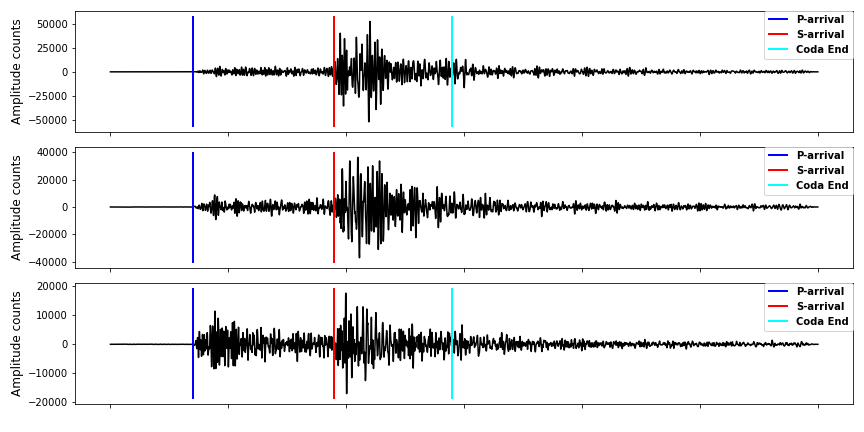
\includegraphics[width=0.9\textwidth]{img/3ch.png}
    \caption{Three channels of seismic wave}
    \label{fig:3-wave}
\end{figure}

The seismic wave includes the body wave that is through the Earth's solid interior, and the surface wave that is a wave that travels along the Earth's surface. The body and surface waves also generate ground shaking, which makes them dangerous to people and important places that should be protected.

A sequence of waves is generated when an earthquake occurs. The body wave can travel faster than the surface wave so the seismic sensors can detect the body wave first. The body wave contains two types of waves; P-wave and S-wave. Figure \ref{fig:3-wave} shows the sequence of waves; P-wave is the first wave, and S-wave is the second wave detected by seismic sensors. In addition, the P-wave is not dangerous, and the S-wave or surface wave makes the most severe ground shaking. Also, the P-wave can predict the dangers of the S-wave and surface waves that travel slower than the P-wave.

The magnitude of the danger of ground shaking is measured with peak ground acceleration (PGA), which is the maximum of absolute magnitude. Typically, PGA appears from the S-wave or surface wave. \cite{chiang2022neural} uses 80 gal as the threshold. If PGA exceeds the threshold, the seismic wave refers to dangerous seismic waves.

The study~\cite{gasparini2007earthquake} has shown a relationship between the pattern of the seismic wave and the PGA. Although the times that earthquakes occur are unpredictable, the signals of ground motions can be classified as dangerous or not\cite{salam2021earthquake}. Figure \ref{fig:p-wave} shows the seismic wave and its P-wave, S-wave, surface wave, and PGA. It is possible to leverage the delay between the traveling of P-wave and surface waves to classify PGA. So, in the EEW system, P-wave can assess PGA as dangerous, and the system will send the earthquake early warning messages.

\begin{figure}[ht]
    \centering
    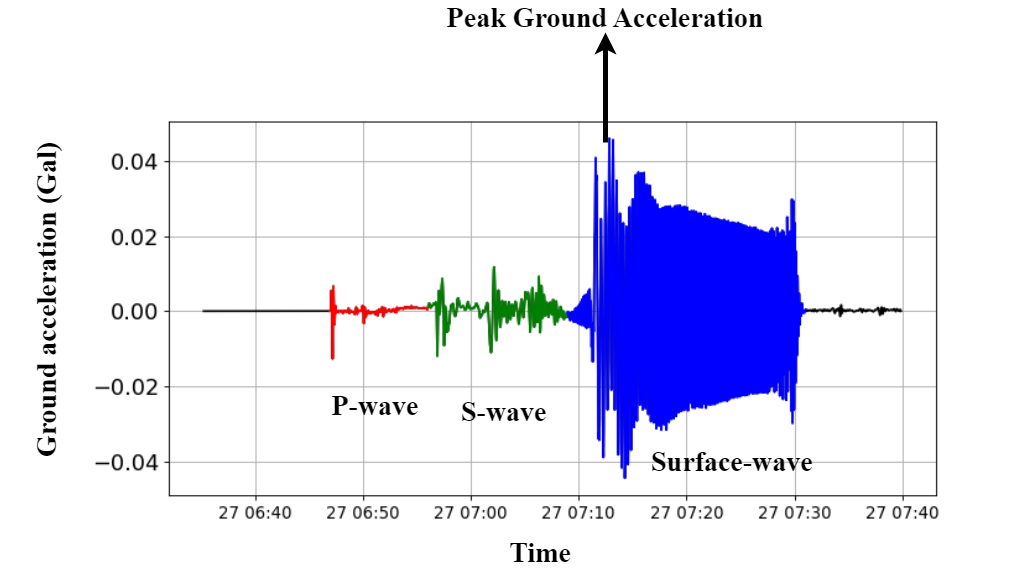
\includegraphics[width=0.9\textwidth]{img/p-wave.png}
    \caption{P-wave, S-wave, Surface-wave, and PGA}
    \label{fig:p-wave}
\end{figure}

\section{The earthquake early warning systems}
%P2. EEW
The Earthquake Early Warning (EEW) system is a way to mitigate people and infrastructure from earthquake disasters. An EEW can provide a warning before ground-shaking, indicating its possible severity. This gives people time to prepare for potential destruction from ground shaking, thereby helping reduce losses. EEW systems are crucial for countries that frequently experience earthquakes. Warnings from these systems can be used in automated systems to prevent destruction from earthquakes. This can apply to transportation services, factories, facilities such as power plants, gas pipelines, and dams, and also assist in alerting people to prepare themselves~\cite{gasparini2007earthquake, allen2019earthquake}. Various countries have advanced early warning systems (e.g. Japan, Mexico, and Taiwan) \cite{gasparini2007earthquake, hsiao2009development}, and sufficient countries are attempting to develop these systems for their countries~\cite{gasparini2007earthquake, allen2019earthquake}.

The earthquake early warning (EEW) systems use the behavior of seismic waves for early warning of the level of danger of seismic waves, and the systems have a model that can predict or classify PGA from a P-wave.

When an earthquake happens, the EEW system helps people to prepare to protect themself. The system manages and shuts down machines, elevators, or trains. The warning from the systems can auto-start things like ceasing transportation services or factories, looking out for some facilities (such as power plants, gas pipelines, and dams), and alerting people affected by the earthquake to prevent themselves \cite{gasparini2007earthquake, allen2019earthquake}. Therefore, the system can mitigate the loss from the earthquake.

% The way to protect people and infrastructures from earthquake disasters is the EEW system which can decrease the destruction from ground shaking.  Various countries have advanced early warning systems for Japan, Mexico, and Taiwan \cite{gasparini2007earthquake, hsiao2009development}, and sufficient countries are attempting to develop these systems for their countries \cite{gasparini2007earthquake, allen2019earthquake}. Thus the EEW systems are crucial for countries that experience earthquake disasters. 
 
% Although EEW systems are a crucial method that helps people from earthquakes, the systems need to retrain models frequently to maintain performance because new earthquake events happen over time. The installations of new seismic sensors also generate new signal data that the systems need to determine. Additionally, the model must manipulate multiple channels of seismic wave data. 

% Furthermore, the model must be adapted and trained to ensure they work for specific characteristics of the zone in which they work. Many new seismic sensors are installed over time, leading to models of EEW systems that should constantly be retrained. That means the high-performance early warning system needs a signal analytic approach or model that is fast and precise. Moreover, a good model for EEW uses low computational consumption and fast training, while the model can maintain high performance.

% Therefore, the systems require a model that can manipulate the multiple time series data and retrain frequently. 

\section{Models}
The appropriate model used in the EEW systems should be fast, precise, and low computational consumption. There are various research proposed models to assess PGA by P-wave. The models 
can be separated into three types:
\begin{enumerate}
    \item The mathematical models provided by experts.
    \item The machine learning models that models are built from preprocessed data.
    \item Deep learning models that models learn by raw data directly.
\end{enumerate}

 Experts design the mathematical models, but they are suitable for some local areas, and they may have a bias from the human. 
 
 The machine learning models make predictions based on data, so they do not have bias and are precise. The machine learning models work well with structured data, but the seismic waves are unstructured data. So, the preprocessing data is required to transform the raw wave data into some parameters that the mathematical model may process. That makes the models work slowly.

The deep learning models can extract the practicable features from the raw data directly. They can find the complex relationship between features and use them to predict or classify the data labels—this is why deep learning is powerful. Some deep-learning models can also work with multi-channel time series data like a seismogram. Therefore, it is interesting for researchers to apply deep learning with the EEW systems.


\subsection{Deep learning in EEW systems}
% In recent years, deep learning methods have been used to apply to monitor earthquakes. The advantages of the deep learning method are that they do not need experts to model them, but their learning is based on data. The research attempts to use various deep learning structures, for example, basic artificial neural network (ANN),  long-short-term memories (LSTM), and convolutional neural network (CNN) such as \cite{chiang2022neural, jozinovic2020rapid, li2018machine, mousavi2020machine}. Various countries, including Japan, Mexico, Taiwan, Italy, and the USA, have researchers who investigate and apply deep learning models to EEW systems \cite{gasparini2007earthquake, hsiao2009development}. 

%P3. DL in EEW
In recent years, deep-learning methods have been used to monitor earthquakes. The advantages of the deep learning method are that they do not require experts to model them, but their learning is based on data. Researchers attempted to use various deep learning structures, such as basic artificial neural networks (ANN),  long short-term memories (LSTM), and convolutional neural networks (CNN)~\cite{chiang2022neural, jozinovic2020rapid, li2018machine, mousavi2020machine}. Various countries have research that investigates and applies deep learning models to EEW systems~\cite{gasparini2007earthquake, hsiao2009development}.

\subsection{Limitations of the deep learning in EEW systems}
%P4. DL problems
%4.1 computational resource
However, the deep learning models used in EEW are large and require vast resources for training the models. The EEW systems require high computational resources for real-time processing of data transmitted from seismometer networks, which are used to detect ground shaking~\cite{wu2021crowdquake+}. An EEW system that uses the deep learning model incurs immense computational costs for training and classification~\cite{li2018machine}.

%4.2 retrain
Although EEW systems are a crucial method that helps people avoid the danger of earthquakes, the systems need to retrain models frequently to maintain performance because new earthquake events occur over time. The installation of new stations also generates new signal data that the systems must determine, and the model must manipulate multiple channels of seismic wave data. Therefore, these systems require models that can manipulate multiple time series data and retrain frequently.

Furthermore, the deep learning models must be adapted and trained to ensure they work for specific characteristics of the land zone in which they are located. Moreover, new seismic stations are installed over time, leading to models of EEW systems that should always be retrained. That means the high-performance early warning system needs a signal analytic approach or model that is fast and precise. 

Moreover, a good model for EEW uses low computational consumption, and fast training, while the model can maintain high accuracy.

Deep learning and machine learning models are known for faster computation than conventional models. This characteristic makes them highly suitable for integrating into Early Earthquake Warning (EEW) systems\cite{anikiev2022traveltime, maharjan2022deep,  lim2022leqnet, wu2021crowdquake+}. Nevertheless, deep learning and machine learning models still demand intensive processing power despite their fast computation. It becomes challenging when optimizing them for deployment on small devices commonly used in EEW systems. The limitation necessitates using smaller, more lightweight models to ensure practical and effective implementation\cite{wu2021crowdquake+, lim2022leqnet}.

Also, the EEW systems need to retrain models frequently to maintain performance because new earthquake events happen over time, and there are the installations of new stations that collect new signal data that the systems need to determine\cite{anikiev2022traveltime}. Therefore, the systems require a model that can manipulate the multiple time series data and retrain frequently\cite{anikiev2022traveltime, maharjan2022deep}. That means the high-performance early warning system needs a signal analytic approach or model that is fast and precise. Moreover, a good model for EEW uses low computational consumption, and fast training, while the model can maintain high performance\cite{anikiev2022traveltime}.

% \section{Extreme Learning Machine}
% Conventional Artificial Neural Networks using forward–backward algorithms need much training time \cite{lian2013displacement}. The Extreme Learning Machine (ELM) is a single-layer feed-forward network (SLFN). The input weight of this model is fixed (not necessary to train), and the pseudo-inverse matrix optimizes the output weight of the model. The ELM runs faster than classical ANN and can maintain high accuracy \cite{asim2017earthquake, salam2021earthquake}. Also, the ELM runs faster than classical ANN and can maintain high accuracy \cite{asim2017earthquake, salam2021earthquake}.

% \section{Echo State Network}
% This research proposes the Multi-channels Echo State Extreme Learning Machine (Multi ES-ELM). This model is combined between the Echo State Network (ESN) model, which is one type of Reservoir Computing (RC), and the Extreme Learning Machine. The research's model is designed to train with multiple time series data because the seismic wave data has three data channels. Moreover, the model is trained by the extreme learning machine. The model performs almost as well as the CNN model, requiring fewer resources. 



\section{Research Objective}
The EEW system requires a model to classify the PGA from the seismic waves. Furthermore, this model should exhibit key attributes such as efficient training capabilities, real-time processing, rapid classification, and compatibility with multi-channel time series data.

Therefore, the objective of this research is to develop a predictive model for PGA classification utilizing seismic wave data with improved efficiency in terms of retraining time and memory utilization compared to conventional methods. The proposed model combines elements of the ELM model, transitioning from the random linear layer to the ESN for feature extraction.

%P7.
The rest of the paper is organized as follows. Chapter \ref{Chap:relatedwork} discusses related work, focusing on the conventional EEW systems model. In Chapter \ref{Chap:ResearchApproach}, the Multi ES-ELM approach is detailed. Chapter \ref{chap:performance} compares the performance of the proposed Multi ES-ELM model with the CNN model. The final section provides a conclusion to this work.

% The article is separated into three sections. The \ref{sec:relatedwork} section is related work explaining the conventional EEW systems model. The \ref{sec:approch} section shows seismic wave data and how the ESN model is trained and works. Finally, the \ref{sec:performance} section comprises the performance between the proposed Multi ES-ELM model and the CNN model.


%\item \textbf{Some Applications for regression and classification problems}
